
%(BEGIN_QUESTION)
% Copyright 2006, Tony R. Kuphaldt, released under the Creative Commons Attribution License (v 1.0)
% This means you may do almost anything with this work of mine, so long as you give me proper credit
En tank inneholder tre ulike væsker med ulik massetethet. Regn ut trykket som manometeret i bunn av tanken vil vise i Pa og bar. 

$$\includegraphics[width=15.5cm]{i00235x01.eps}$$

$\rho \: glyserin = 1260 kg/m^3$\\
$\rho \: olivenolje = 917 kg/m^3$\\


\underbar{file i00235}
%(END_QUESTION)





%(BEGIN_ANSWER)
$P=97182 Pa$

%(END_ANSWER)





%(BEGIN_NOTES)

See question {\tt i00232.tex} for a list of common fluids' specific gravities.

%INDEX% Physics, static fluids: hydrostatic pressure

%(END_NOTES)


